Matlabb är ett program liknande många andra och består av ett stort
huvudfönster med flikar som skickar dig mellan de olika vyerna. I
figur \ref{fig:oversikt} finns en överblicksbild som visar gränssnittet.

\begin{figure}[h]
        \centering 
        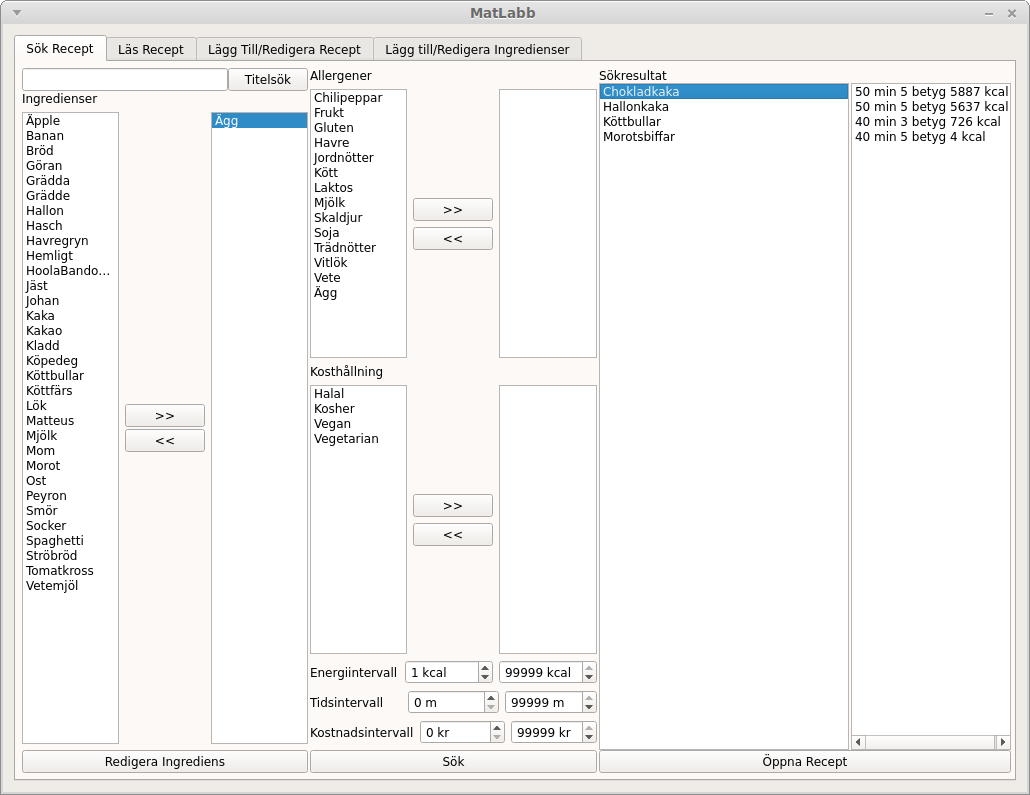
\includegraphics[scale=0.44]{sok_recept.png} 
        \caption{Sökvyn} 
        \label{fig:oversikt}
\end{figure}

För att förflytta sig mellan de olika vyerna behöver man endast klicka
på den berörda fliken och man skickas direkt över.


